\section{Results}\label{sec:results}
Here, I highlight some select few results that were presented in \citet{2023A&A...673A..44F}.

All of the tidal debris from the globular cluster from one galactic potential is shown in Fig.~\ref{fig:LB_count_density}. This highlights that many stellar streams exists, however the tidal debris covers the whole sky and is rather diffuse about the galactic center. 


\begin{figure}
    \centering
    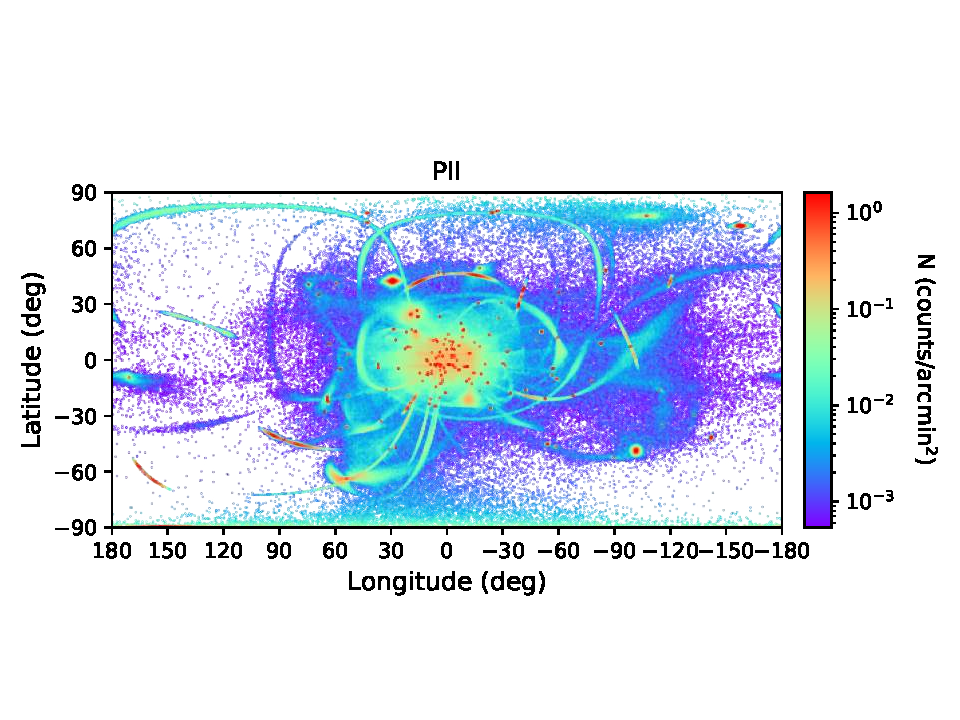
\includegraphics[width=\linewidth,trim={0 2cm 0 2cm},clip]{images/LB_count_density.pdf}
    \caption{The count density of all particles emergent from the 155 globular clustered considered. Many stellar streams are visible as well as general tidal debris crowding the galactic center. Red dots of saturated and high surface density correspond to the positions of the globular clusters. }
    \label{fig:LB_count_density}
\end{figure}

While it is interesting to consider the entire distribution on the sky, it is also interesting to consider the mythologies left by individual clusters. From Fig.~\ref{fig:LB_count_density}, we see that a rich varieities of morhologies are present and not only the thin stellar streams which are commonly championed in the literature. It is instructive to look at the tidal debris resultant from one globular cluster at a time, to get an intuition for the different morphologies that are available. 

In Fig.~\ref{fig:NGC5986}, we show case the orbit and tidal debris of NGC~5986. This is a very instructive example. For instance, recalling the discussion on phase-mixing, we note that this cluster has complete many orbits. As a result, the tidal debris completely occupies all possible states that are accessible to the initial conditions. Note that, in the middle panel, I have colored the recently escaped particles in pink. When truncating to the these particles, we do see that they trace the recent past of the cluster as well as the future leg of the orbit. Thus, even when the tidal debris has been phase-mixed, we can still observe a coherrent stream near a cluster. 

Next, the cluster's tidal debris does not cover the entire sky. This is because the apo-center of the orbit is still within the solar circle. 


\begin{figure}
    \centering
    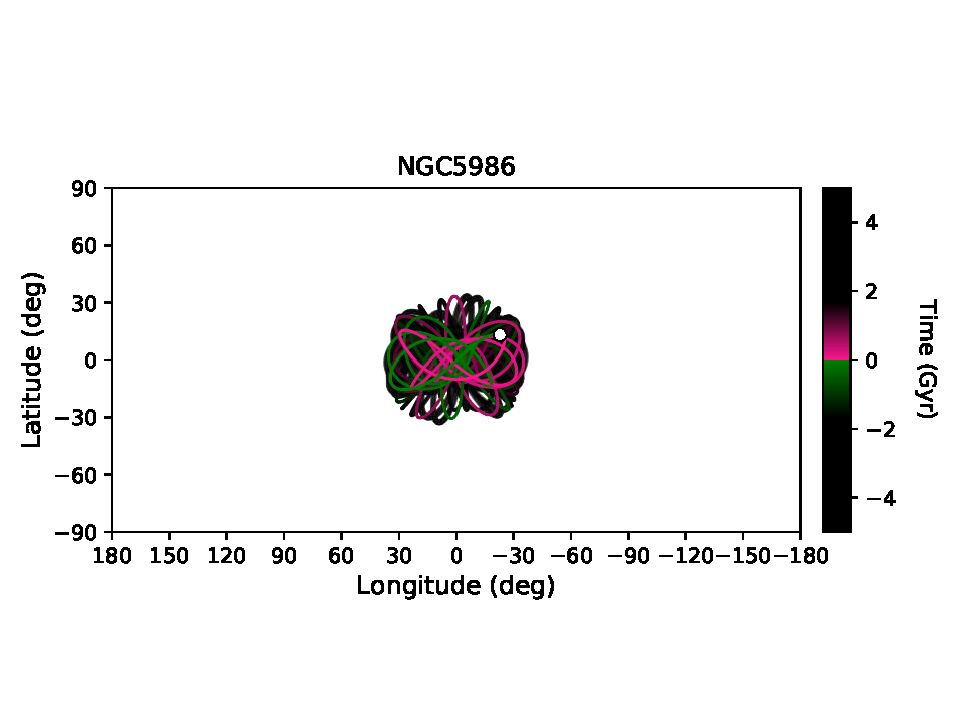
\includegraphics[width=0.9\linewidth,trim={0 3cm 0 2cm},clip]{images/NGC5986orbit.pdf}

    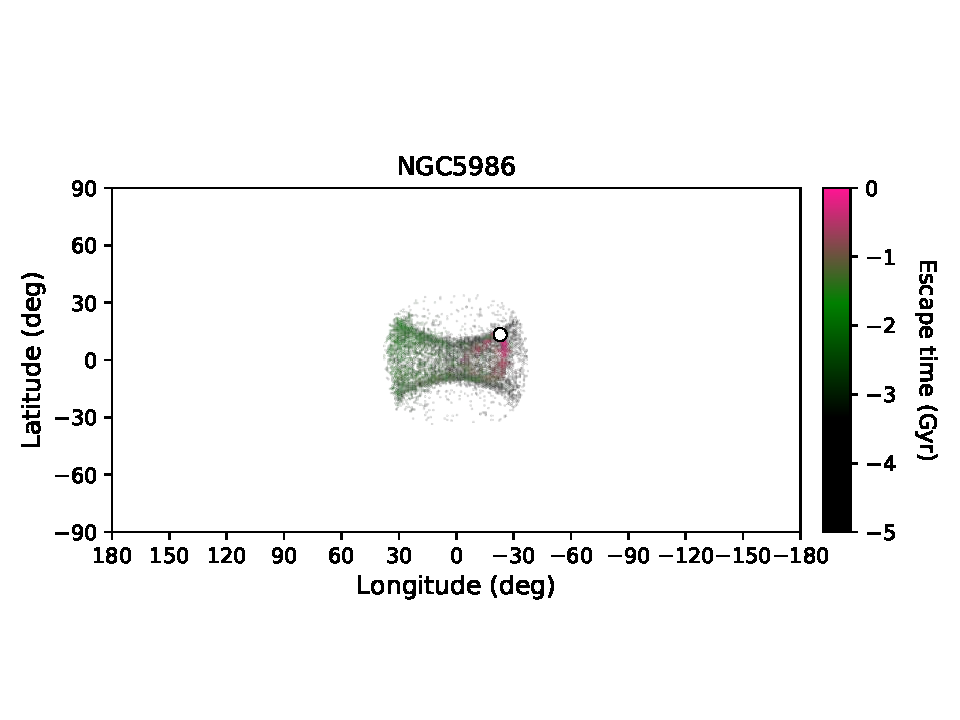
\includegraphics[width=0.9\linewidth,trim={0 2cm 0 3cm},clip]{images/NGC5986_LB_tesc.pdf}

    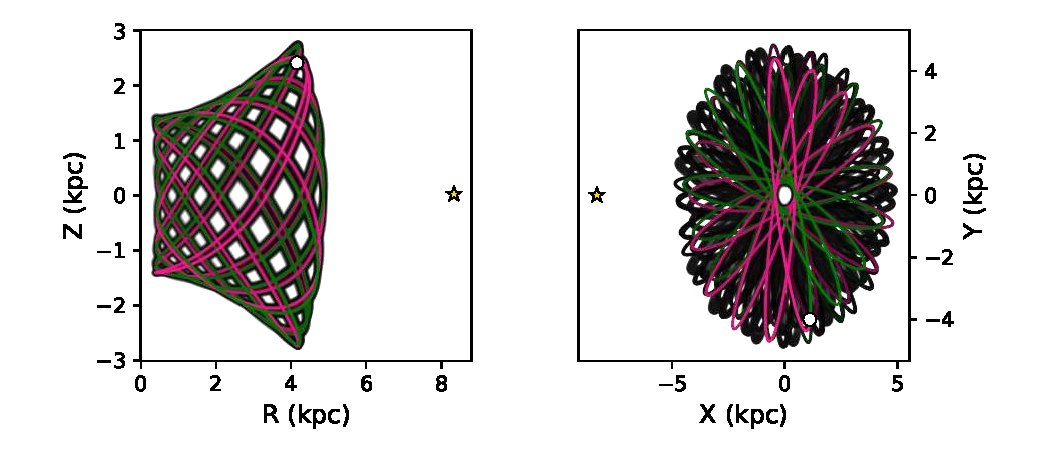
\includegraphics[width=0.9\linewidth]{images/NGC5986orbitRZXY.pdf}    
    \caption{An example case of tidal debris from NGC5986. The top panel shows the orbit in galactic coordinates color coated by time. The white dot shows the position of the cluster today. The middle panel shows the tidal debris colored coated by escape time. The bottom panel shows the orbit in galacto-centric coordinates, with the same colorbar as the top panel. In the bottom panel, the location of the Sun is given by the yellow star.   }
    \label{fig:NGC5986}
\end{figure}

A final interesting note that I wish to discuss in this report, as any good numerical modeler should do, is compare our results to the observations. Fig.~\ref{fig:NGC4590} shows tracks of the same stellar stream compiled from three different studies within \citet{2023MNRAS.520.5225M}. We have remarkable agreement for much of the length of the stream. Notice that our stream goes beyond the observations. This is because the observations are limited. Stellar crowding and extinction in the galactic-mid plane render observations difficult in this region. 

Additionally, notice that the model prediction of the stream of the right panel of Fig.~\ref{fig:NGC4590}. This galactic model included a bar. An intriguing result is that this demonstrates that the stellar streams can be used a diagnostic tools on the bar. However, a precise explanation as to why the bar reduces the length of the stream instead of, say, cutting the stream, still eludes me. 
\begin{figure}
    \centering
    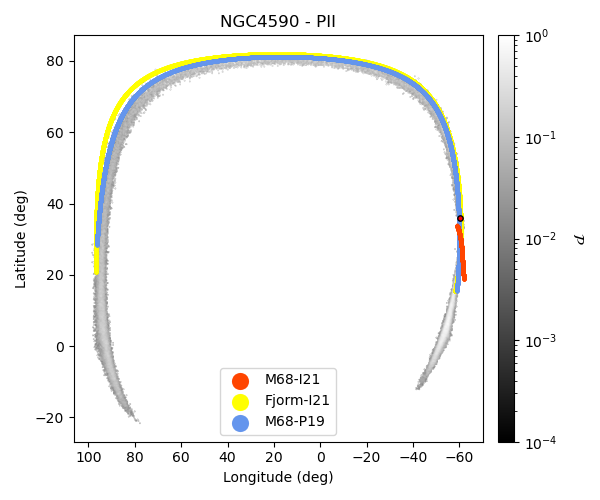
\includegraphics[width=0.45\linewidth]{images/galstream-NGC4590-l-b-pii.png}
    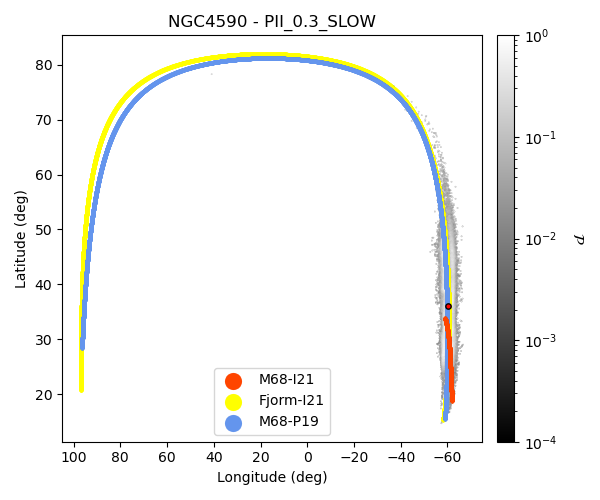
\includegraphics[width=0.45\linewidth]{images/galstream-NGC4590-l-b.png}
    \caption{Two select results from \citep{2023A&A...673A..44F}. Each case shows the tidal debris from the globular cluster NGC4590. The gray probability density map comes from our models. The red, yellow, and blue tracks come from various determinations from the literature and were assembled in \citet{2023MNRAS.520.5225M}. The left panel shows a time static Milky Way potential, while the right shows a model that includes a stellar bar. Notice the right model agrees less with the observation.}
    \label{fig:NGC4590}
\end{figure}


\section{Future work}

We want to include more realistic and complex phenomena within the Galactic field to study how this would impact the tidal debris originating from globular clusters. Several paths of investigation are available to us: the stellar bar, the effects of the Magellanic clouds, the in-fall of Sagittarius, giant molecular clouds, dark matter halos, etc. As a first step, we modified the code to allow for the globular clusters to interact with one another. This experiment is nearly finished and ready for a publication. To summarize here, in step 1 of our methods as described in section~\ref{sec:MinimumWorkingExample}, we integrate the globular clusters with N-Body interactions. Then, in step 2, we allows the star-particles of a given globular cluster feel the gravitational force of all the globular clusters in the galaxy as well as its host and the galaxy. The results are promising, we have assembled a near complete first draft of a letter focusing on a specific analysis of Palomar 5. Then, we wish to expand the work to all globular clusters in the publication of a full article. 

After which, there are three paths that I wish to continue pursuing. (1) including more physics in the simulations. (2) searching for more stellar streams in the real data using the simulation results as a prior. (3) implementing stellar evolution and internal dynamics in the code so that we can create mock-observations. 

Thank you for taking the time to read this report. I look forward to returning to you with more results. 

